\documentclass{mwart}
\usepackage{polski}

\setlength{\emergencystretch}{2em}
\usepackage{datetime}
\usepackage{ae,aecompl}
\usepackage[activate={true,nocompatibility},final,tracking=true,kerning=true,spacing=true,stretch=10,shrink=10]{microtype}
\frenchspacing

%%% fix for \lll
% \let\babellll\lll
% \let\lll\relax
\usepackage{geometry}
\newgeometry{vmargin={25mm}, hmargin={25mm,25mm}}
\usepackage[]{algorithm2e}


\usepackage{enumitem}
\usepackage{graphicx}
\usepackage[normalem]{ulem}
\usepackage{tikz}

\usetikzlibrary{external}
\tikzexternalize[prefix=tikz/]

\usetikzlibrary{arrows.meta}
\usetikzlibrary{matrix, arrows}
\usepackage{program}
\usepackage{amsfonts}
\usepackage{amssymb}
%%% fix for \lll
\let\mathlll\lll
\let\lll\babellll

\usepackage{amsmath}
\usepackage{amsthm}
\usepackage{tikz-cd}
\usepackage{float}
\usepackage{hyperref}
\usepackage{multicol}
\usepackage{mathtools}

\usepackage{array}
\usepackage{wrapfig}
\usepackage{multirow}
\usepackage{tabularx}
\newcommand{\RR}{\mathbb{R}}
\newcommand{\CC}{\mathbb{C}}
\DeclarePairedDelimiter\abs{\lvert}{\rvert}%

\newcommand{\fC}{{\mathfrak C}}
\newcommand{\cM}{{\mathcal M}}
\newcommand{\cC}{{\mathcal C}}
\newcommand{\cD}{{\mathcal D}}
\newcommand{\bN}{{\mathbf{N}}}
\newcommand{\bR}{{\mathbf{R}}}
\newcommand{\bZ}{{\mathbf{Z}}}
\newcommand{\bF}{{\mathbf{F}}}
\newcommand{\bQ}{{\mathbf{Q}}}
\newcommand{\bC}{{\mathbf{C}}}
\newcommand{\cA}{{\mathcal A}}
\newcommand{\cO}{{\mathcal O}}
\newcommand{\cF}{{\mathcal F}}
\newcommand{\cB}{{\mathcal B}}
\newcommand{\Ob}{{\mathrm{Ob}}}
\newcommand{\topl}{\mathcal T}
\newcommand{\Set}{{\mathrm{Set}}}
\newcommand{\Grp}{{\mathrm{Grp}}}
\newcommand{\AbGrp}{{\mathrm{AbGrp}}}
\newcommand{\Mod}{{\mathrm{Mod}}}
\newcommand{\Ring}{{\mathrm{Ring}}}
\newcommand{\Vect}{{\mathrm{Vect}}}
\newcommand{\Alg}{{\mathrm{Alg}}}
\newcommand{\restr}{\mathord{\upharpoonright}}
\newcommand{\liff}{\mathrel{\leftrightarrow}}
\newcommand{\limplies}{\mathrel{\rightarrow}}
\newcommand{\fset}[1]{\left\{{#1}\right\}}
\newcommand{\meet}{\mathbin{\wedge}}
\newcommand{\biglor}{\bigvee}
\newcommand{\bigland}{\bigwedge}


\DeclareMathOperator{\round}{{round}}
\DeclareMathOperator{\cl}{{cl}}
\DeclareMathOperator{\Id}{{Id}}
\DeclareMathOperator{\id}{{id}}
\DeclareMathOperator{\Aut}{{Aut}}
\DeclareMathOperator{\End}{{End}}
\DeclareMathOperator{\Ult}{{Ult}}
\DeclareMathOperator{\Homeo}{{Homeo}}
\DeclareMathOperator{\dom}{{dom}}
\DeclareMathOperator{\rng}{{rng}}
\DeclareMathOperator{\Core}{{Core}}
\DeclareMathOperator{\Hom}{{Hom}}
\DeclareMathOperator{\Stab}{{Stab}}
\DeclareMathOperator{\dcl}{{dcl}}
\DeclareMathOperator{\acl}{{acl}}
\DeclareMathOperator{\tp}{{tp}}
\DeclareMathOperator{\characteristic}{{char}}



\newtheorem{twr}{Twierdzenie}[section]
\newtheorem{hip}[twr]{Hipoteza}
\newtheorem{pyt}[twr]{Pytanie}
\newtheorem{problem}[twr]{Problem}
\newtheorem{lem}[twr]{Lemat}
\newtheorem{fkt}[twr]{Fakt}
\newtheorem{wnsk}[twr]{Wniosek}
\newtheorem{stw}[twr]{Stwierdzenie}
\newtheorem{cw}[twr]{Ćwiczenie}

\theoremstyle{remark}
\newtheorem{uwg}[twr]{Uwaga}
\theoremstyle{definition}
\newtheorem{dfn}[twr]{Definicja}
\newtheorem*{rozw}{Rozwiązanie}
\newtheorem*{sbclm}{Podclaim}
\newtheorem*{clm*}{Claim}
\newtheorem{pd}[twr]{Przykład}
\newcounter{claimcounter}[twr]
\newenvironment{clm}{\stepcounter{claimcounter}{\noindent {\textbf{Claim}} \theclaimcounter:}}{}
\newenvironment{clmproof}[1][\proofname]{\proof[#1]\renewcommand{\qedsymbol}{$\square$(claim)}}{\endproof}
\newenvironment{sbclmproof}[1][\proofname]{\proof[#1]\renewcommand{\qedsymbol}{$\square$(subclaim)}}{\endproof}

\newcommand{\xqed}[1]{%
	\leavevmode\unskip\penalty9999 \hbox{}\nobreak\hfill
	\quad\hbox{\ensuremath{#1}}}
\theoremstyle{definition}
\newtheorem{zad}[twr]{Zadanie}

\title{Pracownia z analizy numerycznej \\
        \large Sprawozdanie do zadania \textbf{P1.10} \\
        Prowadzący: dr Rafał Nowak}
\author{Franciszek Malinka, Kacper Solecki}
\date{Wrocław, Listopad 2020}

\begin{document}

\maketitle

\section{Wstęp}
Funkcje trygonometryczne mają szerokie zastosowania w matematyce, informatyce, inżynierii, architekturze, produkcji muzyki i wielu innych dziedzinach. Nietrudno zatem dojść do wniosku, że ich efektywne i dokładne obliczanie jest problemem bardzo ważnym w kontekście tych zagadnień.

W niniejszym sprawozdaniu przyjrzymy się dwóm opracowanym przez nas metodom obliczania wybranych funkcji trygonometrycznych używając jednie najprostszych operacji arytmetycznych ($+$, $-$, $*$, $/$, ale też przesunięcia bitowe), ze szczególnym naciskiem na dokładne obliczanie funkcji $\sin$ oraz $\cos$, również w dziedzinie liczb zespolonych.

Proponowane przez nas metody mają docelowo dawać poprawne obliczenia dla podwójnej precyzji obliczeń, jednakże testy numeryczne przeprowadzamy używając zmiennych typu \texttt{BigFloat} w języku \texttt{Julia} (w którym implementowaliśmy nasze rozwiązania). Typ ten oferuje dowolną dokładność obliczeń. Wyniki naszych funkcji porównujemy z funkcjami bibliotecznymi języka i zakładamy, że dają one dokładne wyniki.

\section{Algorytm CORDIC}
\subsection{Opis algorytmu}

Pierwszą proponowaną przez nas metodą obliczania funkcji $\sin$ oraz $\cos$ jest Algorytm CORDIC (\textbf{CO}ordinate \textbf{R}otation \textbf{DI}gital \textbf{C}omputer). Algorytm ten został stworzony z myślą o komputerach o niskiej mocy obliczeniowej, ale również o możliwości ''włożenia'' algorytmu w hardware (tj. pozwala tworzyć mało skomplikowane układy bramek logicznych, które obliczają funkcje trygonometryczne). Jak się przekonamy, proces iteracyjny algorytmu korzysta jedynie z dodawania, odejmowania, przesunięć bitowych i wartości obliczonych podczas preprocessingu oraz nie wykorzystuje liczb zmiennoprzecinkowych.

Zacznijmy od wprowadzenia zarysu działania algorytmu. Zapomnijmy na razie o analizie numerycznej i przenieśmy się do świata algebry liniowej. Wyobraźmy sobie, że mamy wydajny system który obliczy wektor $(x_r, y_r)$ jako wynik obrotu danego wektora $(x_0, y_0)$ o dany kąt $\theta$ wokół środka układu współrzędnych:
\begin{align}
  x_r = x_0\cos\theta - y_0\sin\theta, \\
  y_r = x_0\sin\theta + y_0\cos\theta.
\end{align}

Jeśli za $(x_0, y_0)$ weźmiemy punkt $(1, 0)$, to po obrocie dostaniemy:
\begin{align*}
  x_r = \cos\theta, \\
  y_r = \sin\theta.
\end{align*}
Zatem używając obrotu umiemy policzyć wartości funkcji $\cos$ oraz $\sin$.

Zapiszmy równania $(1), (2)$ w formie macierzowej:
\begin{align}
  \begin{bmatrix}
    x_r \\ y_r
  \end{bmatrix}
  = \begin{bmatrix}
    \cos\theta & -\sin\theta \\
    \sin\theta & \cos\theta
  \end{bmatrix}
  \begin{bmatrix}
    x_0 \\ y_0
  \end{bmatrix}
  = \cos\theta
  \begin{bmatrix}
    1          & -\tan\theta \\
    \tan\theta & 1
  \end{bmatrix}
  \begin{bmatrix}
    x_0 \\ y_0
  \end{bmatrix}.
\end{align}

Powyższa równość pokazuje, że do obliczenia naszego wektora wynikowego (przy założeniu, że znamy wartości $\tan\theta$ oraz $\cos\theta$) wystarczą jedynie 4 mnożenia i kilka dodawań lub odejmowań. Chcielibyśmy pozbyć się tych mnożeń. Skorzystamy tutaj z dwóch obserwacji:
\begin{itemize}
  \item Każdy kąt $\theta\in [0^{\circ}, 90^{\circ}]$ możemy zapisać jako sumę \textbf{wcześniej ustalonych}, mniejszych (co do modułu) kątów $\theta_i, i \in \{0, ..., n\}$:
        \begin{align}
          \theta = \sum_{i=0}^n \sigma_i\theta_i, \; \sigma_i \in \{-1, 1\}.
        \end{align}
        Dla przykładu, kąt $57.353^{\circ}$ jest sumą kątów
        $45^{\circ}, 26.565^{\circ}, -14.03^{\circ}$ (dobór tych kątów jest nieprzypadkowy, o czym się zaraz przekonamy). 
        Jeśli $\theta$ nie należy do zadanego przez nas przedziału, to możemy ten kąt zmienić korzystając ze wzorów redukcyjnych 
        (o tym więcej w \textsection 3).
  \item Jeśli nasze kąty $\theta_i$ będą dobrane tak, że $\tan\theta_i = 2^{-i}$, to mnożenie przez $\tan\theta_i$ jest niczym innym jak przesunięciem bitowym (w liczbach całkowitych). Dodatkowo okazuje się, że dowolny kąt nie większy niż $90^{\circ}$ da się przybliżyć sumą tak dobranych kątów $\theta_i$, więc da się tymi kątami osiągnąć cel założony w pierwszym punkcie. Dodatkowo im więcej takich kątów wybierzemy, tym dokładniejsze będzie to przybliżenie.
\end{itemize}

Pozostały nam jeszcze mnożenia przez czynnik $\cos\theta$ (który nazwiemy przyrostem). Jeżeli to zignorujemy, to otrzymana rotacja będzie faktycznie obróceniem wektora o kąt $\theta$, ale z dodatkowym przeskalowaniem wektora.

% \begin{center}
%     \begin{tikzpicture}
%     \draw [<->,thick] (0,6) node (yaxis) [above] {$y$}
%         |- (8,0) node (xaxis) [right] {$x$};
%     \draw [->, thick] (0, 0) -- (6, 2) node (v1) [right] {$(x_0, y_0)$}
%     \draw [->, cm={cos(45) ,-sin(45) ,sin(45) ,cos(45) ,(0 cm, 0 cm)}] (0, 0) -- (6,2)
%     % \draw[black, thick, ->] (0,0) -- (10,0);
%     % \draw[black, thick, ->] (0,0) -- (0,8);
%     \end{tikzpicture}
% \end{center}

Przyjrzyjmy się jak dokładnie będzie wyglądać nasz przyrost, jeśli zastosujemy zaproponowane przez nas punkty do obliczania obrotu. Powiedzmy, że chcemy obrócić wejściowy wektor o kąt $57.353^{\circ} = 45^{\circ} + 26.565^{\circ} - 14.03^{\circ}$. Wartości funkcji $\tan$ tych kątów są odwrotnościami potęg dwójki, zatem te kąty spełniają nasze założenie. Pierwsza rotacja o $45^{\circ}$ daje:
\begin{align}
  \begin{bmatrix}
    x_1 \\ y_1
  \end{bmatrix}
  = \cos 45^{\circ}
  \begin{bmatrix}
    1 & -1 \\
    1 & 1
  \end{bmatrix}
  \begin{bmatrix}
    x_0 \\ y_0
  \end{bmatrix}.
\end{align}
Druga rotacja daje:
\begin{align}
  \begin{bmatrix}
    x_2 \\ y_2
  \end{bmatrix}
  = \cos 26.565^{\circ}
  \begin{bmatrix}
    1      & -2^{-1} \\
    2^{-1} & 1
  \end{bmatrix}
  \begin{bmatrix}
    x_1 \\ y_1
  \end{bmatrix}.
\end{align}
Trzecia rotacja:
\begin{align}
  \begin{bmatrix}
    x_3 \\ y_3
  \end{bmatrix}
  = \cos(-14.03^{\circ})
  \begin{bmatrix}
    1       & 2^{-2} \\
    -2^{-2} & 1
  \end{bmatrix}
  \begin{bmatrix}
    x_2 \\ y_2
  \end{bmatrix}.
\end{align}
Łącząc te równania razem dostajemy:
\begin{align}
  \begin{bmatrix}
    x_3 \\ y_3
  \end{bmatrix}
  = \cos 45^{\circ}\cos 26.565^{\circ}\cos(-14.03^{\circ})
  \begin{bmatrix}
    1 & -1 \\
    1 & 1
  \end{bmatrix}
  \begin{bmatrix}
    1      & -2^{-1} \\
    2^{-1} & 1
  \end{bmatrix}
  \begin{bmatrix}
    1       & 2^{-2} \\
    -2^{-2} & 1
  \end{bmatrix}
  \begin{bmatrix}
    x_0 \\ y_0
  \end{bmatrix}.
\end{align}

Zauważmy, że dzięki parzystości funkcji $\cos$ znak poszczególnych kątów nie ma znaczenia dla wartości przyrostu. Z tego snujemy wniosek, że przy ustalonej liczbie iteracji przyrost nie zależy od wyboru kąta $\theta$. Możemy go zatem policzyć i wziąć go pod uwagę dopiero na koniec obliczeń.
\begin{align}
  P = \cos 45^{\circ}\cdot\cos 26.565^{\circ}\cdot\cos 14.03^{\circ}\cdot\ldots \approx 0.6072.
\end{align}
W takim razie, pomijając przyrost $P$ otrzymujemy następujący proces iteracyjny algorytmu CORDIC:
\begin{align}
  x_{i + 1} & = x_{i} - \sigma_i 2^{-i}y_i, \\
  y_{i + 1} & = y_i + \sigma_i 2^{-i}y_i.
\end{align}

Pozostaje jedynie problem znajdowania znaków $\sigma_i$ przy kątach $\theta_i$. Okazuje się jednak, że możemy to robić w bardzo prosty sposób. Niech $z_0 = \theta, \sigma_0 = 1$. W każdym kroku iteracyjnym znak $\sigma_{i + 1}$ dobieramy w następujący sposób -- niech $z_{i}$ będzie równe $\theta - \sum_{k=0}^{i - 1}\sigma_k\theta_k$ (czyli $z_i$ mówi jaki jeszcze nam został kąt do obrócenia, potencjalnie obróciliśmy już za dużo, wtedy $z_i < 0$). Wtedy $\sigma_{i + 1} = sgn(z_i)$. Mamy też $z_{i + 1} = z_{i} - \sigma_i\theta_i = z_{i} - \sigma_i\arctan{2^{i}}$. Błąd przybliżenia po $n$ iteracjach możemy wtedy łatwo policzyć ze wzoru 
\begin{align}
  \theta_{error} = z_n = \theta - \sum_{i=0}^n\sigma_i \theta_i.
\end{align}

Zbierając wszystko razem, proces iteracyjny algorytmu CORDIC wygląda następująco:
\begin{align*}
  x_{i + 1} & = x_{i} - \sigma_i 2^{-i}y_i,    \\
  y_{i + 1} & = y_i + \sigma_i 2^{-i}y_i,      \\
  z_{i + 1} & = z_i - \sigma_i \arctan 2^{-1}.
\end{align*}

Kąty $\theta_i = \arctan{2^{-1}}$ możemy policzyć w preprocessingu i używać jako stałych. Wtedy rezultatem naszych obliczeń będzie $\cos\theta \approx P\cdot x_n$ oraz $\sin\theta \approx P\cdot y_n$. Dodatkowo, gdybyśmy przyjęli $x_0 = 1/P$, to pozbylibyśmy się nawet tego ostatniego mnożenia.

Warto jeszcze zauważyć, że
\begin{align*}
  \frac{1}{\cos(\arctan 2^{-i})} = \sqrt{1 + \frac{1}{2^{2i}}}.
\end{align*}
Możemy ten fakt wykorzystać do dokładniejszego obliczania wartości $P$.

Musimy jeszcze zauważyć, że algorytm działa jedynie dla kątów $\theta$ spełniających
\begin{align*}
  \abs{\theta} \leq \sum_{i=0}^n\theta_i \approx 99.88^{\circ}.
\end{align*}
Zatem dla kątów większych niż $90^{\circ}$ musimy skorzystać ze wzorów redukcyjnych, co dokłada pewnego błędu do naszego wyniku oraz powoduje konieczność wykonania kilku dodatkowych dzieleń i mnożeń.

\subsection{Niespełniona obietnica}
We wstępie powiedzieliśmy, że algorytm będzie korzystał z dodawań, odejmowań i przesunięć bitowych, a do tego używał liczb całkowitych. Dzięki naszemu ustaleniu, że $\arctan\theta_i = 2^{-i}$, wszystkie mnożenia podczas iteracji naszego algorytmu to mnożenia przez potęgi dwójki. Jak możemy to wykorzystać?

Ustalmy $M := 2^{K}$ dla pewnego $K$ (potem je wybierzemy). Teraz każdą spreprocessowaną 
przez nas wartość $T$ (czyli $T$ jest kątem $\theta_i$ lub przyrostem $P$) przyjmiemy 
$T := \round(M \cdot T)$. Chcąc policzyć wartości funkcji trygonometrycznych dla kąta $\theta$, 
uruchomimy nas proces iteracyjny dla $x_0 = \round(M/P)$, $y_0 = 0$, $z_0 = \round(M\cdot\theta)$. 
Zauważmy, że dzięki temu przeskalowaliśmy wszystkie obliczane przez nas wartości o stałą $M$
i zaokrągliliśmy je po to, by móc pracować na liczbach całkowitych. To pozawala na wykorzystanie 
przesunięć bitowych podczas mnożenia przez potęgi dwójki, dzięki czemu znacznie zwiększyliśmy 
wydajność naszego algorytmu. Wtedy, po $n$ iteracjach naszego procesu mamy $\cos\theta \approx x_n/M$
oraz $\sin\theta\approx y_n/M$ (już w arytmetyce zmiennoprzecinkowej).

Zostało nam ustalić wartość $K$. Na pewno chcielibyśmy, aby $K$ było nie większe niż
długość mantysy. Ponadto algorytm ma być dostosowany do mało wydajnych maszyn, dlatego
w naszych analizach pracujemy przy użyciu \texttt{Int32}, zatem nie chcemy żeby $2^K\cdot T$ przekroczyło
zakres \texttt{Int32}. Jednakże kąty $\theta_i$ oraz wartość $P$ są niewielkie, zatem $K = 30$ będzie
odpowiednią wartością.

\section{Wzór Taylora}
\subsection{Opis metody}
Zanim przejdziemy do opisu tej metody, przypomnijmy sobie pewną tożsamość trygonometryczną:
\begin{align}
  \sin z = \sin (x + yi) = \sin x\cosh (y) + i\cos x\sinh(y).
\end{align}
Korzystając z tej tożsamości pozbywamy się konieczności pracowania z liczbami zespolonymi i możemy operować jedynie w zbiorze liczb rzeczywistych.

W tej metodzie wykorzystamy znany analityczny wzór zwany wzorem Taylora. Korzystając z niego możemy wyprowadzić rozwinięcia funkcji trygonometrycznych:

\begin{align*}
  \sin x  & = x - \frac{x^3}{3!} + \frac{x^5}{5!} - \frac{x^7}{7!} + \ldots, \\
  \sinh x & = x + \frac{x^3}{3!} + \frac{x^5}{5!} + \frac{x^7}{7!} + \ldots, \\
  \cos x  & = 1 - \frac{x^2}{2!} + \frac{x^4}{4!} - \frac{x^6}{6!} + \ldots, \\
  \cosh x & = 1 + \frac{x^2}{2!} + \frac{x^4}{4!} + \frac{x^6}{6!} + \ldots. \\
\end{align*}

Obliczanie rozwinięć poszczególnych funkcji jest proste i wyabstrahowaliśmy je do jednej, generycznej funkcji \texttt{TalyorSeries}:
\begin{center}
  \begin{algorithm}[H]
    \SetAlgoLined
    \KwData{x, parity, changeSign, M}
    \KwResult{Obliczenie szeregu Taylora odpowiedniej funkcji trygonometrycznej w punkcie x dla jego pierwszych M niezerowych wyrazów}
    result := 0\;
    elem := 1\;
    \If{parity = 1}{
      elem := x\;  
    }
    i := parity + 1\;
    \While{i $\le$ 2M + parity}{
      result := result + elem\;
      elem :=  elem * changeSign * x * x / (i * (i + 1))\;
      i := i + 2\;
    }
  \end{algorithm}
\end{center}

Algorytm oblicza sumę $\sum_{n=0}^M\sigma_n\frac{x^n}{n!}$, gdzie $\sigma_i \in \{-1, 0, 1\}$. Wartość $\sigma_n$ zależy od wartości parametrów podanych w funkcji: gdzy \texttt{parity} jest równe $0$, wtedy mamy $\sigma_{2k + 1} = 0$, a gdy \texttt{parity} jest równe $0$ mamy $\sigma_{2k} = 0$. Odpowiada to odpowiednio szeregom $\cos x, \cosh x$ oraz $\sin x, \sinh x$. Od parametru \texttt{changeSign} zależy czy chcemy, aby kolejne niezerowe wyrazy obliczanego szeregu zmieniały znak (zmieniamy znak, gdy chcemy obliczać zwykłe funkcje trygonometryczne oraz nie zmieniamy gdy obliczamy funkcje hiperboliczne). 

To daje prostą możliwość obliczania pożądanych przez nas funkcji:

\begin{align*}
  \sin x  & = \texttt{TaylorSeries}(x, 1, -1, M), \\
  \sinh x & = \texttt{TaylorSeries}(x, 1, 1, M),  \\
  \cos x  & = \texttt{TaylorSeries}(x, 0, -1, M), \\
  \cosh x & = \texttt{TaylorSeries}(x, 0, 1, M).
\end{align*}

Zauważmy, że wzór Taylora nadaje się do przybliżania funkcji trygonometrycznych jedynie dla argumentów bliskich $0$. 
Na szczęście możemy sobie z tym poradzić korzystając ze znanych tożsamości trygonometrycznych oraz okresowości funkcji $\sin$ i $\cos$. 
Naszym celem przed obliczniem funkcji \texttt{TaylorSeries} będzie sprowadzenie argumentu do przedziału $[0, \pi/4]$,
w którym wzór Taylora bardzo dobrze przybliża wartości funkcji trygonometrycznych. 
Oto tabela która przedstawia jak radzimy sobie z argumentami spoza tego przedziału:
\begin{table}[H]
  \centering
  \begin{tabular}{ |p{4cm}||p{4cm}|p{4cm}| }
    \hline
    \multicolumn{3}{|c|}{Wzory redukcyjne}                     \\
    \hline
    Warunek na $x$ & $\sin x$            & $\cos x$            \\
    \hline
    $x < 0$        & $-\sin (-x)$        & $\cos (-x)$         \\
    $x \ge 2\pi$   & $\sin(x \mod 2\pi)$ & $\cos (x\mod 2\pi)$ \\
    $x > \pi$      & $-\sin(x - \pi)$    & $-\cos(x - \pi)$    \\
    $x > \pi/2$    & $\cos(x - \pi/2)$   & $-\sin(x - \pi/2)$  \\
    $x > \pi/4$    & $\cos(\pi/2 - x)$   & $\sin(\pi/2 - x)$   \\
    \hline
  \end{tabular}
  \caption{Wzory redukcyjne.}
  \label{tab:reduk}
\end{table}

Dla funkcji hiperbolicznych sposób jest prostszy: korzystamy z dwóch własności:
\begin{align*}
  \sinh x & = 2\sinh(x/2)\cosh(x/2),       \\
  \cosh x & = \cosh^2(x/2) + \sinh^2(x/2).
\end{align*}
Można by przypuszczać, że dla dużych $x$ błąd obliczania tych funkcji będzie duży. Jednakże okazuje się, że funkcje te bardzo szybko rosną i już dla $x = 1000$ wartości obu tych funkcji nie mieszczą się w zakresie \texttt{Float64}, zatem tak naprawdę wykonamy maksymalnie $15$ takich redukcji, co generuje dopuszczalnie mały błąd.

\section{Analiza błędu}

\subsection{Wyniki testów}
Dokładność naszych metod porównywaliśmy z funkcjami bibliotecznymi w języku \texttt{Julia}, które domyślnie obsługują obliczanie wartości funkcji trygonometrycznych dla liczb zespolonych. Zakładmy o tych funkcjach bibliotecznych, że dają poprawny wynik.

Przeprowadziliśmy testy dokładności metody opartej na wzorze Taylora dla liczb rzeczywistych oraz dla liczb zespolonych oraz testy dla metody Taylora, w której nie używaliśmy wzorów redukcyjnych, lecz rozwijaliśmy wzór dopóki wystarczająco dobrze nie przybliżał wartości funkcji dla danego argumentu. Testy dla algorytmu CORDIC przeprowadziliśmy wyłącznie dla liczb rzeczywistych. 

Dla każdej metody przeprowadziliśmy trzy rodzaje testów, w każdym z nich losowaliśmy $10^8$ liczb z różnych przedziałów. Ze względu na podobieństwo funkcji $\sin$ i $\cos$ oraz z faktu, że często wzory redukcyjne powodują faktycznie obliczanie innej funkcji trygonometrycznej, testy przeprowadziliśmy wyłącznie dla funkcji $\sin$. Przedziały i wyniki testów przedstawione są w poniższej tabeli oraz na wykresach:

\begin{table}[H]
  \centering
  \resizebox{\textwidth}{!}{%
    {\setlength{\extrarowheight}{5pt}%
        \begin{tabular}{ |c||c|c|c|c|c| }
          \hline
          algorytm                                                    & przedział argumentu            & średni błąd wz.        & max błąd wz.           & średni błąd bezwz.     & max błąd bezwz.        \\
          \hline
          \multirow{3}{6em}{Taylor dla $\RR$}                         & $x:$ dowolny Float64           & $1,887 \cdot 10^{-15}$ & $3,167 \cdot 10^{-8}$  & $1,179 \cdot 10^{-16}$ & $8,882 \cdot 10^{-16}$ \\
          \cline{2-6}
                                                                      & $-2\pi \leq x \leq 2\pi$       & $1,472 \cdot 10^{-15}$
                                                                      & $1.184 \cdot 10^{-8}$          & $9,766 \cdot 10^{-17}$ & $5,551 \cdot 10^{-16}$                                                   \\ 
          \cline{2-6}
                                                                      & $0 \leq x \leq 1$              & $8,694 \cdot 10^{-17}$ & $6,661 \cdot 10^{-16}$ & $4,293 \cdot 10^{-17}$ & $4,441 \cdot 10^{-16}$ \\
          \hline
          \multirow{3}{6em}{Taylor dla $\CC$}                         & $-100 \leq \abs{x} \leq 100$   & $4,932 \cdot 10^{-15}$ & $1,311 \cdot 10^{-13}$ & $1,689 \cdot 10^{26}$  & $5,898 \cdot 10^{29}$  \\
          \cline{2-6}
                                                                      & $-2\pi \leq \abs{x} \leq 2\pi$ & $4,338 \cdot 10^{-16}$ & $1,487 \cdot 10^{-11}$ & $1,364 \cdot 10^{-14}$ & $8,710 \cdot 10^{-13}$ \\
          \cline{2-6}
                                                                      & $0 \leq \abs{x} \leq 1$        & $1,597 \cdot 10^{-16}$ & $1,099 \cdot 10^{-15}$ & $1,124 \cdot 10^{-16}$ & $1,111\cdot 10^{-15}$  \\
          \hline
          \multirow{3}{6em}{Taylor dla $\CC$ bez wzorów redukcyjnych} & $-100 \leq \abs{x} \leq 100$   & $4,77 \cdot 10^{23}$   & $4,488 \cdot 10^{26}$  & $7,759 \cdot 10^{40}$  & $2,208 \cdot 10^{44}$  \\
          \cline{2-6}
                                                                      & $-2\pi \leq \abs{x} \leq 2\pi$ & $6,333 \cdot 10^{-1}$  & $1,000$                & $2,344 \cdot 10$       & $2,677 \cdot 10^2$     \\
          \cline{2-6}
                                                                      & $0 \leq \abs{x} \leq 1$        & $1,589 \cdot 10^{-16}$ & $1,291 \cdot 10^{-15}$ & $1,118 \cdot 10^{-16}$ & $1,116 \cdot 10^{-15}$ \\
          \hline
          \multirow{3}{6em}{Cordic dla $\RR$}                         & $x:$ dowolny Float64           & $3,100 \cdot 10^{-8}$  & $4,575 \cdot 10^{-1}$  & $2,459 \cdot 10^{-9}$  & $5,529 \cdot 10^{-3}$  \\
          \cline{2-6}
                                                                      & $-2\pi \leq x \leq 2\pi$       & $2,770 \cdot 10^{-8}$  & $1,183 \cdot 10^{-1}$  & $2,532 \cdot 10^{-9}$  & $6,042 \cdot 10^{-4}$  \\
          \cline{2-6}
                                                                      & $0 \leq x \leq 1$              & $4,176 \cdot 10^{-8}$  & $9,182 \cdot 10^{-2}$  & $2,614 \cdot 10^{-9}$  & $5,261 \cdot 10^{-4}$  \\
          \hline
        \end{tabular}
      }}
  \caption{Błędy przy obliczaniu funkcji $\sin(x)$.}
  \label{tab:2}
\end{table}
\clearpage
% \begin{center}

Poniższe wykresy obrazują wielkości błędów względnych obu algorytmów\newline przy liczeniu sinusa w przedziale $[0, 2\pi]$:
\begin{figure}[H]
\centering
    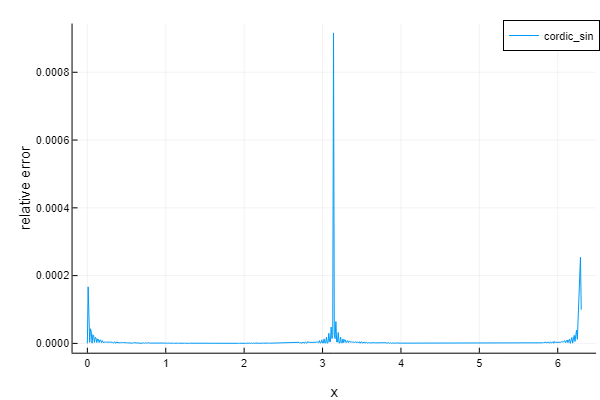
\includegraphics[scale = 0.6]{cordic error.png}
    \caption{Błąd względny algorytmu CORDIC dla wartości funkcji $\sin$}
    \label{rys:1}
\end{figure}
% \end{center}

% \begin{center}
\begin{figure}[H]
\centering
    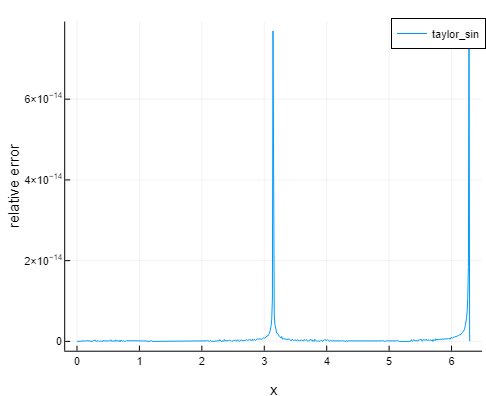
\includegraphics[scale = 0.9]{taylor error.png}
\caption{Błąd względny metody Taylora dla wartości funkcji $\sin$}
\label{rys:2}
\end{figure}
% \end{center}


\subsection{Wnioski}
Jak widać w tabeli \ref{tab:2}, dla wszystkich testów zaproponowane przez nas metody sprawdzają 
się bardzo dobrze dla małych argumentów. Algorytm CORDIC wypada dużo gorzej od metody korzystającej 
ze wzoru Taylora, lecz nie jest to dla nas nic zaskakującego -- metoda ta tworzy kompromis 
między wydajnością, a dokładnością obliczeń. Dla obu metod widać, że problemem jest zmiana 
argumentu na mały, gdyż to generuje duży błąd obliczeń. W obu przypadkach największy błąd względny
generowały argumenty zbliżone do wielokrotności $\pi$, jak widać na rysunkach \ref{rys:1} i \ref{rys:2}. Wynika to z konieczności odejmowania, 
z którego korzysta wbudowana w \texttt{Julia} funkcja \texttt{mod2pi} oraz wzory redukcyjne.
Prowadzi do utraty cyfr znaczących, tym samym obniżając dokładność obliczeń.

Dużym problemem w obliczaniu wartości funkcji trygonometrycznych w dziedzinie liczb zespolonych jest konieczność używa funkcji hiperbolicznych, które rosną w tempie wykładniczym. Jeśli spojrzymy na wzór $(13)$ to zauważmy, że bardzo prawdopodobne jest, że będziemy mnożyć zbliżoną do $0$ wartość funkcji $\sin$ oraz $\cos$ z potencjalnie bardzo dużymi wartościami funkcji $\cosh$ i $\sinh$. 

Mimo to jesteśmy zadowoleni z rezultatów dla losowych testów -- jak widać, średni błąd względny jest rzędu dokładności liczb o precyzji podwójnej w przypadku metody Taylora oraz rzędu pojedynczej precyzji dla algorytmu CORDIC (co wynika z użycia \texttt{Int32} podczas procesu iteracyjnego).

\begin{thebibliography}{9}
  \bibitem{CORDIC tutorial}
  Steve Arar.
  \textit{An Introduction to the CORDIC Algorithm}. 
  \\\texttt{\url{https://www.allaboutcircuits.com/technical-articles/an-introduction-to-the-cordic-algorithm/}}
  
  \bibitem{CORDIC ints}
  Andrea Vitali.
  \textit{Coordinate rotation digital computer algorithm (CORDIC)
    to compute trigonometric and hyperbolic functions}.
  \\\texttt{\url{https://bit.ly/3lVQxbJ}}
\end{thebibliography}
\end{document}